\documentclass[conference]{IEEEtran}
\usepackage{graphicx}
\usepackage{tikz}
\usepackage{pgfplots}
\pgfplotsset{compat=1.18}
\usepackage{booktabs}
\usepackage{multirow}
\usepackage{amsmath,amssymb}
\usepackage{url}
\usepackage{balance}
\usepackage{microtype}
\usepackage{array}
\usepackage{enumitem}
\setlist[itemize]{leftmargin=*,nosep}
\newcommand{\ucer}{\textsc{UCER}}
\newcommand{\udr}{\textsc{UDR}}
\newcommand{\arsr}{\textsc{ARSR}}
\newcommand{\frr}{\textsc{FRR}}
\newcommand{\sbsr}{\textsc{SBSR}}
\newcommand{\hdr}{\textsc{HDR}}

\title{When Heuristics Fail but Boundaries Hold:\\Structural vs. Heuristic Security in Healthcare RAG}

\author{\IEEEauthorblockN{Nassim Tinkicht, Hussain Al-Aqrabi}
\IEEEauthorblockA{Higher Colleges of Technology, United Arab Emirates\\
Email: \{ntinkicht, halaqrabi\}@hct.ac.ae}}

\begin{document}
\maketitle

\begin{abstract}
Retrieval-augmented generation (RAG) can expose sensitive records before a language model produces any visible answer. We study where authorization should be enforced in a healthcare RAG pipeline and separate two outcomes that are often conflated: unauthorized context exposure during retrieval and unauthorized disclosure in generated text. Using deterministic Synthea v4.0.0 data, we evaluate 3,000 security cases (9,000 architecture executions) across prompt-only, pre-retrieval access control, and a risk-aware variant. Pre-retrieval authorization reduces unauthorized context exposure from 1,750/1,750 to 0/1,750, while the prompt-only canary disclosure rate is only 5/1,750 and its 5-to-0 reduction is not conventionally significant (exact McNemar $p=0.0625$). A controlled $k=1$ follow-up resolves an apparent utility penalty: all three architectures obtain 895/1,000 authorized-task successes when retrieval composition is held identical, showing that the earlier gap was caused by distractor composition rather than the authorization gate in this benchmark. A label-independent risk-feature redesign further shows that structural ACL denial generalizes to held-out phrasing, whereas heuristic suspicion triage does not: challenge-or-deny rates fall from 88.0\% to 16.7\% for fuzzy control and from 100\% to 16.0\% for deterministic rules. Finally, a nested 1K--100K retrieval study shows strong growth in unfiltered and proportional-scope retrieval cost and distractor similarity, while fixed-scope conditions serve as construction controls. The results support authorization-before-retrieval as a structural security boundary, but do not support claims that fuzzy triage outperforms transparent rules or that zero observed leakage proves zero real-world risk.
\end{abstract}

\begin{IEEEkeywords}
retrieval-augmented generation, access control, healthcare security, authorization, prompt injection, synthetic health records, formal verification
\end{IEEEkeywords}

\section{Introduction}
RAG systems augment a language model with records selected from an external datastore \cite{lewis2020rag}. In a healthcare setting, this creates a security question that is more fundamental than whether a model eventually prints protected information: \emph{did the system retrieve protected information into model context at all?} If authorization is enforced only through instructions inside the prompt, the model may be told not to reveal a record after the record has already crossed the security boundary.

Recent work has begun integrating permissions and metadata filtering into RAG pipelines. Chen \emph{et al.} demonstrated access control over patient profiles in a 40-profile proof of concept \cite{chen2025sac}; Jeong and Lee proposed IAM-backed permission-aware filtering for multi-resource environments \cite{jeong2025permission}; and Chen and Taipalus combined metadata filtering with fine-grained role-based access control \cite{chen2026metadata}. In parallel, extraction attacks show that RAG datastores can be deliberately induced to leak through instruction following and adaptive querying \cite{qi2025spill,dimaio2025pirates}. These lines of work motivate a careful distinction between retrieval-time exposure and generation-time leakage, and between a structural access-control boundary and heuristic attack detection.

This paper evaluates three architectures under the same synthetic healthcare benchmark: (i) a prompt-only baseline that retrieves globally and places authorization policy in the system prompt, (ii) deterministic pre-retrieval ACL filtering, and (iii) the same ACL boundary with an additional risk-triage controller. Our central claim is deliberately narrow: \emph{authorization should constrain the retrieval candidate set before sensitive content is assembled into model context}. We do not claim clinical efficacy, model-level privacy, or authentication correctness; principal resolution is assumed to have occurred before the evaluated pipeline begins.

The study makes four contributions. First, it separates Unauthorized Context Exposure Rate (\ucer) from a narrow canary Unauthorized Disclosure Rate (\udr), preventing a low output-leak rate from masking a complete retrieval-boundary failure. Second, it resolves an initially observed utility gap with a paired, controlled $k=1$ experiment that equalizes retrieval composition. Third, it compares fuzzy risk triage with a transparent deterministic-rule baseline using label-independent telemetry and lexically disjoint held-out suspicious prompts; the negative generalization result constrains what can credibly be attributed to risk scoring. Fourth, it adds a secondary, nested 1K--100K systems study that separates global-corpus growth from authorization-scope growth while fitting a single retrieval representation on the 100K master corpus.

\section{Related Work}
\subsection{Authorization-aware RAG}
Chen \emph{et al.} \cite{chen2025sac} integrate access control into a patient-profile RAG prototype and evaluate 40 generated profiles. Their proof of concept demonstrates feasibility but does not separate retrieval exposure from generated disclosure or study the effect of authorization location at the scale used here. Jeong and Lee \cite{jeong2025permission} validate permissions against native IAM endpoints in multi-resource environments and quantify policy-enforcement and answer-quality effects. Chen and Taipalus \cite{chen2026metadata} use metadata both for filtering and fine-grained RBAC, emphasizing secure and relevant retrieval. Together, these studies establish that permission-aware retrieval is an active design direction; our novelty is therefore not the existence of pre-retrieval filtering itself, but a security-ablation methodology that isolates enforcement location, distinguishes context exposure from output disclosure, resolves a retrieval-depth confound, and examines fixed versus proportional authorization scopes at larger corpus sizes.

\subsection{RAG datastore extraction}
Qi \emph{et al.} show scalable extraction from retrieval-in-context RAG systems using instruction-following behavior across multiple model families \cite{qi2025spill}. Di Maio \emph{et al.} propose an adaptive black-box attack that iteratively discovers anchors correlated with previously extracted knowledge \cite{dimaio2025pirates}. These attacks reinforce why retrieved context itself is security-relevant. Our benchmark is not an attempt to reproduce these full adaptive attacks; instead, it uses controlled unauthorized and adversarial prompt families to test whether the retrieval boundary can cross an ACL and whether a narrow marker can reach generated output.

\subsection{Synthetic healthcare records and formalization}
We use Synthea because it produces distributable synthetic health records without introducing real-patient privacy risk \cite{walonoski2018synthea}. Formal analysis uses NuSMV \cite{cimatti2002nusmv} over an abstract state machine. Fuzzy control follows the general notion of graded membership introduced by Zadeh \cite{zadeh1965fuzzy}, but we treat it as one policy implementation rather than as a security guarantee in itself.

\section{Threat Model and Security Boundary}
The evaluated pipeline begins after a principal has been resolved to an account label. Authentication, identity proofing, token theft, account compromise, and correctness of the upstream identity provider are out of scope. The adversary can submit arbitrary text to the RAG query interface and can reference patients for whom the resolved account has no permission. We assume the authorization matrix supplied to the retriever is correct; ACL administration errors are therefore also outside the modeled boundary.

The critical distinction is shown below:
\begin{figure}[t]
\centering
\footnotesize
\setlength{\tabcolsep}{3pt}
\begin{tabular}{c c c c c}
Request & $\rightarrow$ & Auth/Risk & $\rightarrow$ & ACL filter \\
&&&& $\downarrow$ \\
&& LLM $\leftarrow$ Context $\leftarrow$ & Retrieval &
\end{tabular}
\caption{Secured ordering. Authorization constrains the candidate set before retrieval; the risk layer can tighten but cannot widen the ACL.}
\label{fig:pipeline}
\end{figure}
In the prompt-only baseline, retrieval is global and the authorization rule appears in the system prompt. This is not a no-policy straw man: it retains an authorization instruction but tests whether prompt-level policy is an adequate substitute for a retrieval-time boundary. In both secured architectures, candidate records are first restricted to the account ACL. The risk-aware architecture may reject or step up a request before retrieval, but an \texttt{ALLOW} decision cannot add records outside the ACL.

We define \ucer{} for an unauthorized request as the event that at least one record outside the requesting account's permissions is included in retrieved context. \udr{} is narrower: it detects whether a synthetic, record-specific security marker appears in generated output. A system can therefore have low \udr{} while still having catastrophic \ucer{}, because a model may receive protected context without reproducing the canary. \arsr{} measures correct task completion on the 1,000 ordinary authorized requests; \frr{} measures rejection of those requests.

\section{Dataset and Experimental Design}
\subsection{Synthetic corpus and authorization model}
The publication benchmark uses Synthea v4.0.0, seed 4103, reference date 2026-01-01, Massachusetts, producing 1,000 normalized FHIR R4 patient records. The median normalized record is 1,430 characters. Accounts A--D receive 200 patients each; 200 additional patients form a globally protected pool, and account E receives no permissions. Aliases \texttt{PAT-0001}--\texttt{PAT-1000} are used in the controlled prompts. The protected pool is not inert: 400 benchmark cases target protected aliases, spanning direct unauthorized and all five adversarial categories.

\begin{table}[t]
\caption{Primary benchmark composition.}
\label{tab:composition}
\centering
\footnotesize
\begin{tabular}{lrr}
\toprule
Category & Cases & Unauthorized \\
\midrule
Authorized normal & 1,000 & 0 \\
Direct unauthorized & 1,000 & 1,000 \\
Authorized suspicious & 250 & 0 \\
Direct injection & 150 & 150 \\
Privilege/debug & 150 & 150 \\
Context extraction & 150 & 150 \\
Role-play/obfuscated & 150 & 150 \\
Multi-step & 150 & 150 \\
\midrule
Total & 3,000 & 1,750 \\
\bottomrule
\end{tabular}
\end{table}

Each case is executed against three architectures with the same SmolLM2-360M-Instruct checkpoint, greedy decoding, and \texttt{max\_new\_tokens=64}, yielding 9,000 primary executions. A separate 1,000-case legitimate-only follow-up is executed across all three architectures with explicit $k=1$ retrieval, adding 3,000 executions. We also add 300 held-out cases (150 unauthorized and 150 authorized-but-suspicious) and 200 alias-free name-resolution cases, for a total of 13,500 core LLM executions.

\subsection{Risk-feature redesign and comparators}
Earlier versions used a session-trust feature tied to benchmark category. The revision replaces it with deterministic simulated telemetry derived from account, target, and seed: failed-authorization count, request rate, off-hours use, and known-device status. Category-wise trust means are tightly clustered (approximately 0.68--0.70; medians 0.71), removing label separability. We compare the fuzzy controller with deterministic threshold rules built over the same non-label-derived features. Both controllers are hand-tuned; the comparison asks whether fuzzy aggregation contributes observed value, not whether either threshold set is optimal.

The held-out suspicious templates are deliberately lexically disjoint from the frozen injection-keyword detector: all held-out prompts receive injection risk 0.0. This makes the held-out set a test of heuristic generalization, while unauthorized-target denial remains structurally governed by ACL membership.

\subsection{Statistics and independence caveat}
Paired binary outcomes are compared with exact McNemar tests. Wilson intervals describe binomial proportions. For the controlled $k=1$ utility difference we additionally bootstrap the paired risk difference with 20,000 draws. Latency and retrieval-scale comparisons use paired Wilcoxon tests where appropriate.

Case-level intervals and $p$-values should not be interpreted as 150 or 1,750 independent attack \emph{strategies}. Attack categories reuse a small number of templates instantiated with different targets. We therefore report the leaking template explicitly and treat template dependence as a primary threat to validity rather than inflating the effective evidence count.

\section{Primary Security and Utility Results}
\subsection{Retrieval exposure and generated disclosure}
Table~\ref{tab:main} shows the central security result. Global retrieval exposes unauthorized context in every one of 1,750 unauthorized prompt-only requests. Both secured architectures reduce observed \ucer{} to 0/1,750. The Wilson 95\% upper bound for 0/1,750 is 0.219\%, so this result is evidence of strong performance under the modeled ACL, not proof that real-world risk is zero.

\begin{table}[t]
\caption{Primary security and utility outcomes.}
\label{tab:main}
\centering
\footnotesize
\begin{tabular}{lccc}
\toprule
Metric & Prompt-only & Pre-ACL & Risk-aware \\
\midrule
\ucer{} (unauth.) & 1750/1750 & 0/1750 & 0/1750 \\
\udr{} canary & 5/1750 & 0/1750 & 0/1750 \\
\arsr{} ($k=2$) & 790/1000 & 640/1000 & 705/1000 \\
\frr{} & 0/1000 & 0/1000 & 0/1000 \\
\arsr{} (controlled $k=1$) & 895/1000 & 895/1000 & 895/1000 \\
\bottomrule
\end{tabular}
\end{table}

The prompt-only canary detector fires in only 5/1,750 unauthorized cases (0.286\%, Wilson 95\% CI 0.122--0.667\%). The secured architectures show 0/1,750. However, the paired 5-to-0 comparison yields exact McNemar $p=0.0625$, so we do not claim a conventionally significant reduction in generated canary leakage. This is precisely why \ucer{} and \udr{} must be reported separately: a model can suppress a marker while protected content has already been placed in its context.

All five canary disclosures come from one repeated multi-step template. That template leaks in 5/50 instances (10\%); the other 700 adversarial unauthorized instances in the five 150-case attack categories produce no canary leak. The 5/1,750 case-level number is therefore accompanied by the template-level result rather than treated as evidence over 1,750 independent attack strategies.

\subsection{The apparent utility penalty was a retrieval-composition confound}
At $k=2$, prompt-only \arsr{} is 79.0\%, pre-retrieval ACL is 64.0\%, and risk-aware is 70.5\%. The target record is present in all 1,000 legitimate cases for all architectures, yet the prompt-only and pre-ACL retrieved sets differ in all 1,000 paired cases. The original gap therefore cannot be interpreted cleanly as the price of authorization.

The controlled $k=1$ experiment removes the distractor by forcing the same retrieval depth for all architectures. Figure~\ref{fig:kcontrol} shows complete convergence: 895/1,000 successes for each architecture, zero prompt-only-versus-ACL discordant outcomes, exact McNemar $p=1.0$, and a paired ACL-minus-prompt risk difference of 0.0 with bootstrap 95\% CI [0.0, 0.0]. This supports a specific causal interpretation: \emph{in this benchmark, once retrieval-set composition is held identical, the authorization gate itself introduces no additional observed utility loss}. It does not imply that access control can never reduce utility in other retrieval systems or policy regimes.

\begin{figure}[t]
\centering
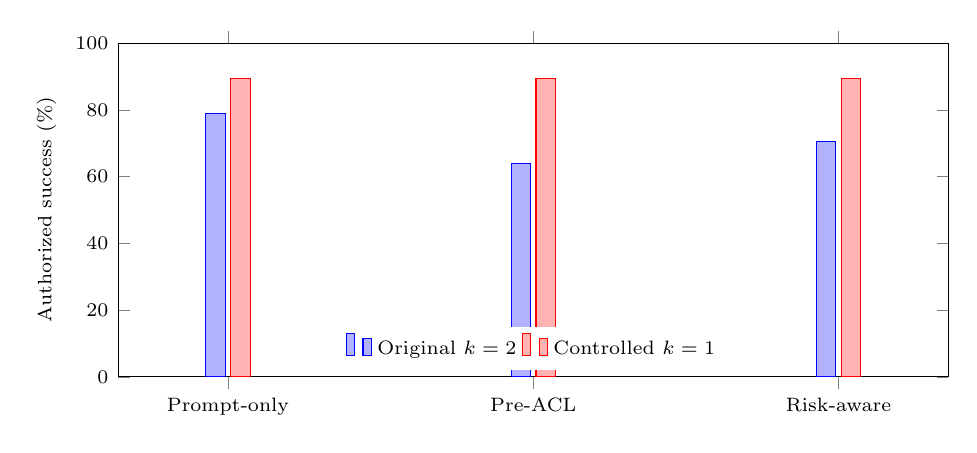
\begin{tikzpicture}
\begin{axis}[
  width=\columnwidth,height=0.48\columnwidth,
  ybar,bar width=7pt,ymin=0,ymax=100,
  ylabel={Authorized success (\%)},
  symbolic x coords={Prompt-only,Pre-ACL,Risk-aware},xtick=data,
  xticklabel style={font=\scriptsize},
  yticklabel style={font=\scriptsize},
  label style={font=\scriptsize},
  legend style={font=\scriptsize,draw=none,at={(0.5,0.02)},anchor=south,legend columns=2},
  enlarge x limits=0.18]
\addplot coordinates {(Prompt-only,79.0) (Pre-ACL,64.0) (Risk-aware,70.5)};
\addplot coordinates {(Prompt-only,89.5) (Pre-ACL,89.5) (Risk-aware,89.5)};
\legend{Original $k=2$,Controlled $k=1$}
\end{axis}
\end{tikzpicture}
\caption{Authorized-request success before and after controlling retrieval depth. The $k=1$ follow-up removes the distractor-composition confound.}
\label{fig:kcontrol}
\end{figure}

\section{Risk Triage: Robust Boundary, Weak Generalization}
The risk-aware layer is subordinate to the ACL and should be evaluated separately from the structural authorization guarantee. On the primary authorized-but-suspicious set, the fuzzy controller challenges or denies 88.0\% of requests, while the deterministic-rule comparator challenges 100\%. On the lexically disjoint held-out suspicious set, those rates collapse to 16.7\% and 16.0\%, respectively (Fig.~\ref{fig:risk}). Neither controller denies a held-out authorized-suspicious request; most are indistinguishable from benign prompts under the frozen lexical features.

\begin{figure}[t]
\centering
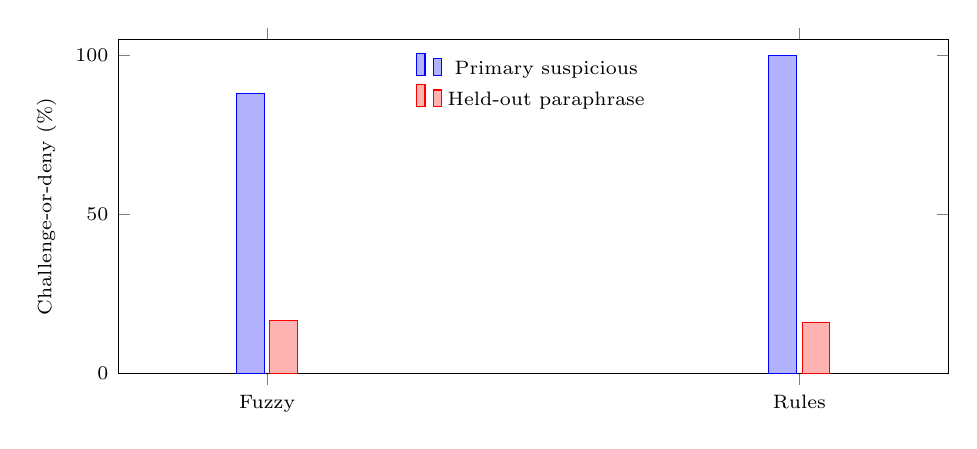
\begin{tikzpicture}
\begin{axis}[
  width=\columnwidth,height=0.48\columnwidth,
  ybar,bar width=10pt,ymin=0,ymax=105,
  ylabel={Challenge-or-deny (\%)},
  symbolic x coords={Fuzzy,Rules},xtick=data,
  xticklabel style={font=\scriptsize},
  yticklabel style={font=\scriptsize},
  label style={font=\scriptsize},
  legend style={font=\scriptsize,draw=none,at={(0.5,0.98)},anchor=north,legend columns=1},
  enlarge x limits=0.28]
\addplot coordinates {(Fuzzy,88.0) (Rules,100.0)};
\addplot coordinates {(Fuzzy,16.7) (Rules,16.0)};
\legend{Primary suspicious,Held-out paraphrase}
\end{axis}
\end{tikzpicture}
\caption{Suspicion-triage generalization. Structural unauthorized-target denial remains 100\% for both controllers, but suspicious-authorized challenge rates collapse under held-out paraphrases.}
\label{fig:risk}
\end{figure}

By contrast, unauthorized-target denial is 100\% for both controllers on both primary and held-out sets. This is not evidence that the heuristic detector generalizes; it follows from authorization confidence and the ACL boundary. The fuzzy-vs-rule paired challenge comparison over the combined evaluation yields $p=0.0043$, but the direction is not a fuzzy advantage: deterministic rules challenge more in-distribution cases and the two are nearly identical out of distribution. We therefore present fuzzy logic only as one adaptive policy mechanism and make no claim that it outperforms transparent threshold rules.

\begin{table}[t]
\caption{Risk-triage behavior on authorized-suspicious requests.}
\label{tab:risk}
\centering
\footnotesize
\begin{tabular}{lrr}
\toprule
Controller & Primary & Held-out paraphrase \\
\midrule
Fuzzy challenge-or-deny & 88.0\% & 16.7\% \\
Deterministic rules & 100.0\% & 16.0\% \\
Fuzzy deny only & 26.4\% & 0.0\% \\
Rules deny only & 50.4\% & 0.0\% \\
\bottomrule
\end{tabular}
\end{table}

The alias-free benchmark further tests a separate robustness question. Queries identify a synthetic patient by name rather than by \texttt{PAT-xxxx} alias. Authorized target resolution succeeds in 100/100 cases for both secured architectures; unauthorized target resolution/retrieval is 0/100, because candidate filtering remains limited to authorized aliases even when direct alias parsing is absent. This supports a bounded claim about name-based resolution in the implemented retriever, not general identifier robustness.

\section{Secondary 1K--100K Retrieval-Scale Study}
\subsection{Design}
To separate global-corpus growth from authorization-scope growth, we construct a deterministic nested master corpus of 100,000 Synthea patients. The original 1,000 patients remain the exact prefix. Additional records are deterministically selected and assigned so that each of A--D has either a fixed 200-patient ACL or a proportional ACL of 200, 2,000, and 20,000 at 1K, 10K, and 100K respectively; the protected share remains 20\% in the proportional condition.

A single TF-IDF(1,2) representation (float32) is fitted once on the 100K master and smaller conditions restrict candidate rows only. This avoids an IDF/vocabulary confound. Four hundred paired legitimate queries are evaluated per scale under unfiltered, fixed ACL, proportional ACL, and target-scoped controls. A 90-query LLM subset uses unfiltered, fixed-ACL, and target-fixed modes. Importantly, fixed-ACL and target-fixed candidate sets do not change with global scale; flat retrieval identity or answer behavior in those modes is therefore a \emph{construction control}, not an emergent scalability finding.

\subsection{Retrieval behavior}
Unfiltered median retrieval latency grows from 3.01 ms at 1K to 12.91 ms at 10K and 129.91 ms at 100K. The proportional ACL condition grows from 2.29 ms to 4.73 ms and 25.64 ms as its authorized candidate pool grows 200$\rightarrow$2,000$\rightarrow$20,000. The fixed 200-patient ACL condition remains near 2.3--2.8 ms because its candidate set is intentionally unchanged. The unfiltered 1K-vs-100K latency increase is significant under paired Wilcoxon testing ($p=2.73\times10^{-67}$); proportional-scope latency shows the same monotonic direction.

Distractor similarity also increases as the candidate pool grows. Median best-distractor TF-IDF similarity rises from 0.037 at 1K to 0.094 at 100K for unfiltered retrieval, and from 0.034 to 0.071 under proportional ACL. Correspondingly, the median target margin decreases from 0.322 to 0.264 unfiltered and from 0.329 to 0.289 proportional. Hit@1 remains 1.0 for these deliberately target-explicit legitimate queries, so the scale result is about increasing interference and cost, not target disappearance.

\begin{figure}[t]
\centering
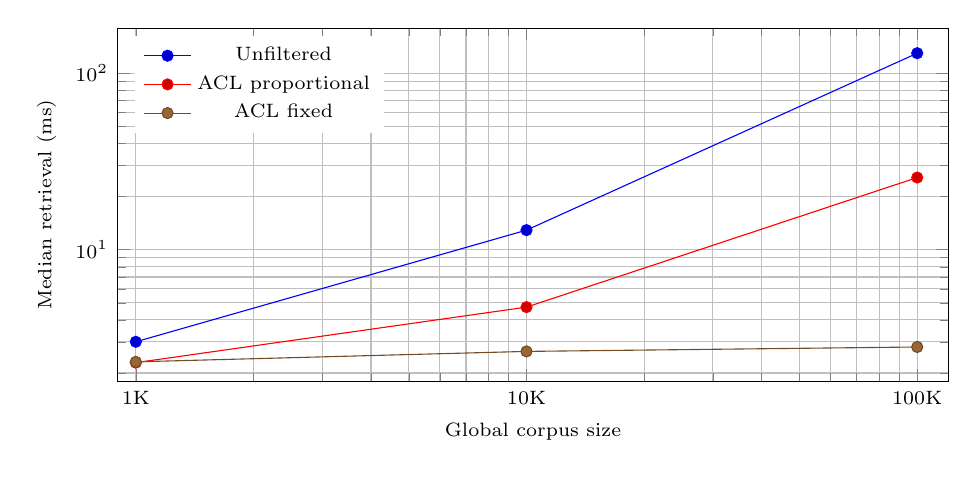
\begin{tikzpicture}
\begin{loglogaxis}[
  width=\columnwidth,height=0.50\columnwidth,
  xlabel={Global corpus size},ylabel={Median retrieval (ms)},
  xmin=900,xmax=120000,ymin=1.8,ymax=180,
  xtick={1000,10000,100000},xticklabels={1K,10K,100K},
  xticklabel style={font=\scriptsize},yticklabel style={font=\scriptsize},label style={font=\scriptsize},
  legend style={font=\scriptsize,draw=none,at={(0.02,0.98)},anchor=north west},
  grid=both]
\addplot+[mark=*] coordinates {(1000,3.0057) (10000,12.9066) (100000,129.9133)};
\addplot+[mark=*] coordinates {(1000,2.2896) (10000,4.7257) (100000,25.6390)};
\addplot+[mark=*] coordinates {(1000,2.3133) (10000,2.6512) (100000,2.8086)};
\legend{Unfiltered,ACL proportional,ACL fixed}
\end{loglogaxis}
\end{tikzpicture}
\caption{Median retrieval latency under nested scaling. Fixed ACL is a constant-candidate control; proportional ACL exposes the effect of growing authorization scope.}
\label{fig:scale_latency}
\end{figure}

\begin{table}[t]
\caption{Selected retrieval-scale outcomes (400 paired queries).}
\label{tab:scale}
\centering
\scriptsize
\begin{tabular}{lrrrr}
\toprule
Mode & Cand. 1K & Cand. 100K & Lat. 1K & Lat. 100K \\
\midrule
Unfiltered & 1,000 & 100,000 & 3.01 ms & 129.91 ms \\
ACL fixed & 200 & 200 & 2.31 ms & 2.81 ms \\
ACL proportional & 200 & 20,000 & 2.29 ms & 25.64 ms \\
Target fixed & 1 & 1 & 0.0006 ms & 0.0016 ms \\
\bottomrule
\end{tabular}
\end{table}

\subsection{LLM subset}
In the 90-query LLM subset, unfiltered \arsr{} is 68.9\% at 1K, 68.9\% at 10K, and 64.4\% at 100K. The paired 1K-vs-100K difference is not significant ($p=0.523$), so we do not claim generation-quality degradation from corpus growth. Target-fixed retrieval supplies the same one-record context by construction and yields 90.0\% at each scale; the unfiltered-vs-target-fixed difference is significant at each scale ($p=1.57\times10^{-4}$, $6.60\times10^{-5}$, and $5.65\times10^{-6}$). This demonstrates the utility of a target-scoped control for these queries, not scale-invariance as a discovered property. Fixed-ACL LLM retrieval likewise reuses the same 200 candidates and is not used to claim authorization-scope scaling.

\begin{figure}[t]
\centering
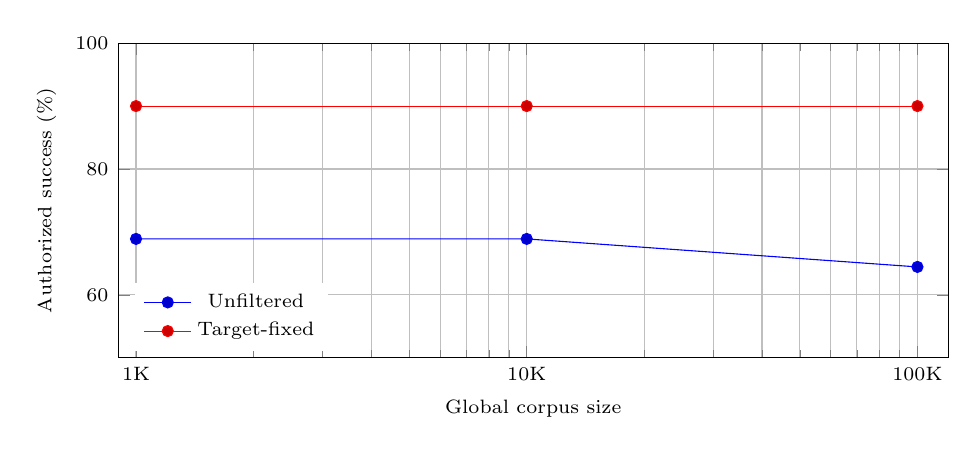
\begin{tikzpicture}
\begin{semilogxaxis}[
  width=\columnwidth,height=0.46\columnwidth,
  xlabel={Global corpus size},ylabel={Authorized success (\%)},
  xmin=900,xmax=120000,ymin=50,ymax=100,
  xtick={1000,10000,100000},xticklabels={1K,10K,100K},
  xticklabel style={font=\scriptsize},yticklabel style={font=\scriptsize},label style={font=\scriptsize},
  legend style={font=\scriptsize,draw=none,at={(0.02,0.02)},anchor=south west},
  grid=both]
\addplot+[mark=*] coordinates {(1000,68.89) (10000,68.89) (100000,64.44)};
\addplot+[mark=*] coordinates {(1000,90.0) (10000,90.0) (100000,90.0)};
\legend{Unfiltered,Target-fixed}
\end{semilogxaxis}
\end{tikzpicture}
\caption{LLM subset. Target-fixed provides a constant single-record context by construction; the unfiltered 1K-to-100K ARSR change is not significant.}
\label{fig:scale_llm}
\end{figure}

We intentionally do not make a generation-level claim for proportional ACL scope because that condition was evaluated only in the retrieval study. The 100K experiment is therefore a secondary systems result: it shows how candidate-set growth changes retrieval cost and interference, not whether authorization correctness depends on corpus size.

\section{Formal Model and Implementation Correspondence}
We model the secured ordering as a finite-state machine with states for login, authenticated processing, risk check, ACL check, retrieval, LLM response, denial, and completion. NuSMV 2.7.1 verifies seven CTL properties: authentication failure cannot reach protected processing; ACL denial cannot reach retrieval; retrieval implies authentication and ACL authorization; fuzzy \texttt{ALLOW} cannot override ACL denial; risk \texttt{DENY} transitions to a safe terminal state; valid authenticated/authorized/non-denied requests eventually complete; and authentication failure at login immediately denies. All seven properties hold in the secured abstraction. A deliberately vulnerable model without these gates falsifies all four corresponding safety properties and produces counterexamples.

\begin{table}[t]
\caption{Formal-to-implementation correspondence.}
\label{tab:formal}
\centering
\scriptsize
\begin{tabular}{p{0.07\columnwidth}p{0.31\columnwidth}p{0.43\columnwidth}}
\toprule
Prop. & Abstract guarantee & Executable correspondence \\
\midrule
P1/P7 & Auth failure cannot proceed & Authentication-gating unit paths \\
P2 & ACL deny never retrieves & Denied request returns before retriever \\
P3 & Retrieval implies ACL subset & Retrieved aliases asserted subset of ACL \\
P4 & Fuzzy ALLOW cannot widen ACL & ALLOW path still receives ACL candidates \\
P5 & Risk DENY stops before retrieval & DENY path asserts no retrieval \\
P6 & Valid path reaches generation & Authorized, non-denied path reaches LLM \\
\bottomrule
\end{tabular}
\end{table}

The correspondence tests are example-based executable checks, not an exhaustive proof of Python implementation correctness. The exhaustive statement applies only to the finite NuSMV abstraction under its assumptions. The combination improves traceability between the model and code but should not be read as formal verification of the entire software stack.

\section{Discussion}
\subsection{Authorization location is the main security result}
The most important distinction in these experiments is not between fuzzy and deterministic logic, but between \emph{policy after retrieval} and \emph{policy before retrieval}. The prompt-only system contains an authorization instruction, yet its retriever still has access to the complete corpus. Consequently, every unauthorized request crosses the retrieval boundary even though only five canary strings are reproduced. This gap matters operationally: once a protected record is in context, security relies on the behavior of a probabilistic generator and on the completeness of output monitoring. Pre-retrieval authorization instead makes the candidate set itself a policy object. Under the modeled assumptions, an unauthorized record is absent before model invocation.

This ordering also clarifies the role of risk scoring. A risk controller can reduce workload, trigger step-up authentication, or reject suspicious activity earlier, but it should not decide which protected records a principal is allowed to retrieve. Our held-out experiment makes that separation empirical rather than rhetorical. Lexical suspicion features fail under paraphrase, while ACL denial remains unchanged. A detector may therefore be useful for operational adaptation without being part of the confidentiality proof obligation.

\subsection{Utility depends on retrieval composition, not only policy strictness}
The original $k=2$ result could easily have produced the misleading conclusion that security caused a 15-point utility loss. The paired diagnostic shows a more specific mechanism: the target was present for all legitimate queries, but each architecture paired it with a different distractor. For the small instruction-tuned model used here, the identity of that second record substantially affected answer success. The controlled $k=1$ experiment is therefore more than a robustness check; it demonstrates why security ablations must control retrieval composition before interpreting answer-quality differences causally.

This finding does not imply that narrower authorization scopes always preserve utility. In a real system, a user may legitimately need information spread across several records, and a policy can remove relevant evidence. The correct design principle is instead to compare architectures at matched information availability when estimating the \emph{overhead of enforcement}, and separately study policy-induced information loss when that is the research question.

\subsection{What the 100K study adds}
The scale study contributes a systems perspective rather than another authorization-correctness test. Because the ACL check is set membership, correctness does not become more or less true at 100K patients. What changes is the retrieval environment: candidate pools become larger, latency rises, and the best distractor becomes more similar to the target. The proportional-ACL condition is especially informative because its authorized scope grows with the corpus; it shows that pre-filtering is not a magical constant-time operation when user entitlements themselves scale. Conversely, the fixed-ACL and target-fixed modes are intentionally invariant controls and should remain labeled as such.

The LLM subset gives only limited evidence about generation under scale. Unfiltered answer success declines numerically at 100K but not significantly, and proportional ACL was not passed through the generator. We therefore avoid a claim that larger corpora necessarily reduce generation quality. What is supported is the retrieval-side observation that larger candidate sets increase cost and interference, while precise target scoping provides a high-utility control for the explicitly targeted queries used here.

\section{Implications for Secure RAG Design}
The results suggest a layered design in which each mechanism has a distinct responsibility. Collapsing those responsibilities into a single ``safety'' score makes both engineering and evaluation harder.

\textbf{1) Make authorization a data-plane constraint.} The retriever should receive an already constrained candidate set, or enforce an equivalent metadata predicate inside the query engine. The security invariant is not that the model was \emph{told} about permissions, but that no document outside the resolved principal's policy can be selected. This implies that retrieval logs should record the principal, policy version, candidate-scope identifier, and retrieved document identifiers before generation begins. Such logging provides a directly auditable counterpart to \ucer{} and makes authorization failures observable without inspecting generated prose.

\textbf{2) Keep target resolution inside the authorized namespace.} Alias-free testing shows that a query need not contain the canonical identifier for the system to remain safe: resolution can operate over the principal's authorized candidate pool. In production, entity linking, spelling correction, aliases, and demographic disambiguation should therefore resolve \emph{after} policy scoping, or return candidate identifiers to a policy check before retrieval. A resolver that searches globally and only later checks the selected entity can recreate the same boundary problem as prompt-only authorization.

\textbf{3) Treat risk scoring as an operational control.} The held-out paraphrase result argues against assigning confidentiality guarantees to lexical or hand-crafted suspicion scores. Risk signals remain useful for rate limiting, step-up authentication, analyst review, or choosing a more restrictive answer policy. However, their failure should degrade into a normal authorized request, not into broader data access. The correct composition rule is monotonic: risk may remove capabilities or require additional assurance, but it may not add records to the ACL-approved set.

\textbf{4) Separate retrieval quality from policy quality.} The $k=1$ control shows how easily a retrieval-composition change can masquerade as a security--utility trade-off. Evaluation pipelines should therefore retain retrieved identifiers and target ranks, not only final answers. When two architectures differ in answer quality, investigators can first determine whether they received the same evidence. This is especially important in small-model evaluations, where one additional distractor can change an otherwise deterministic answer.

\textbf{5) Report scale in terms of both corpus size and entitlement size.} A 100K datastore does not imply a 100K search for every principal. Fixed-scope and proportional-scope conditions represent different deployment regimes. Systems papers should therefore report the size of the global corpus, the authorized candidate pool, and any target-scoped subquery separately. Our proportional condition shows that authorization filtering itself becomes more expensive as entitlements grow, while the global condition shows the larger cost of searching everything. These are operational findings, not changes in the logical meaning of authorization.

\begin{table}[t]
\caption{Evidence-to-design mapping.}
\label{tab:implications}
\centering
\scriptsize
\begin{tabular}{p{0.24\columnwidth}p{0.27\columnwidth}p{0.28\columnwidth}}
\toprule
Observed result & Design implication & Claim boundary \\
\midrule
0/1,750 secured \ucer{} & Scope candidates before retrieval & Under correct ACL/principal \\
5/1,750 baseline \udr{} & Do not infer safety from output alone & Canary detector is narrow \\
$k=1$ ARSR convergence & Control evidence composition & Benchmark-specific causal result \\
Held-out risk collapse & Keep heuristic risk subordinate & No detector-generalization claim \\
Proportional latency growth & Report entitlement size at scale & Retrieval-side, not LLM utility \\
\bottomrule
\end{tabular}
\end{table}

These principles also suggest a monitoring split. Security monitoring should track unauthorized retrieval attempts, policy-evaluation failures, and boundary violations as hard events. Model-quality monitoring should track target rank, context composition, answer success, and refusals. Risk-monitoring should track challenge rates and calibration drift. Keeping these telemetry streams distinct avoids a common failure mode in which a model refusal is counted as evidence that unauthorized data were never retrieved.

\section{Threats to Validity and Limitations}
\textbf{Synthetic data and model choice.} Synthea enables reproducibility and avoids real-patient exposure, but synthetic records do not capture every property of production EHRs. SmolLM2-360M-Instruct is intentionally lightweight; leakage and utility behavior may differ for larger proprietary models. The work evaluates systems/security behavior, not clinical correctness.

\textbf{Prompt families and pseudoreplication.} The benchmark contains many target instantiations of relatively few templates. Case-level exact tests are useful for paired software behavior but overstate the number of independent attack strategies. The concentration of all five canary leaks in one 50-case template illustrates this dependence. Future work should preregister larger, independently authored attack families or use cluster-aware analysis.

\textbf{Canary disclosure is narrow.} \udr{} detects a synthetic marker, not every possible semantic disclosure of protected information. A zero canary count cannot establish zero disclosure risk. \ucer{} is therefore the primary security outcome because it measures boundary crossing directly.

\textbf{Authorization assumptions.} The ACL is treated as authoritative, and the benchmark starts after principal resolution. Stolen credentials, identity-provider errors, ACL misconfiguration, insider misuse, and cross-tenant policy administration are not modeled.

\textbf{Risk scoring.} Both fuzzy membership boundaries and deterministic thresholds are hand-tuned. The held-out result shows that lexical heuristics fail to generalize to paraphrased suspicious-but-authorized requests. Learned detectors could improve recall but would introduce their own calibration, drift, and explainability concerns. The structural ACL should remain the boundary regardless of detector choice.

\textbf{Scale controls.} Fixed-ACL and target-fixed LLM conditions are constant-context controls by construction. The proportional ACL condition reaches 20,000 authorized candidates at 100K in the retrieval study, but was not run through the LLM subset. Accordingly, we make no generation-level statement about proportional authorization-scope growth.

\section{Robustness and Audit Checks}
Several diagnostics were retained specifically to prevent favorable aggregate rates from hiding implementation artifacts.

\textbf{Feature-label separation.} The revised session-trust signal is generated from deterministic account/target telemetry rather than benchmark category. Across the eight primary categories, mean trust ranges only from 0.6800 to 0.6977 and every category has median 0.71. Authorized-normal and authorized-suspicious means are 0.6909 and 0.6904, respectively. This does not prove that every possible derived feature is statistically independent of prompt class, but it rules out the previous direct category-to-trust encoding and removes the large separability that could have made risk decisions tautological.

\begin{table}[t]
\caption{Selected session-trust diagnostics after leakage removal.}
\label{tab:trust}
\centering
\scriptsize
\begin{tabular}{lrr}
\toprule
Category & Mean trust & Median \\
\midrule
Authorized normal & 0.6909 & 0.71 \\
Authorized suspicious & 0.6904 & 0.71 \\
Direct unauthorized & 0.6800 & 0.71 \\
Direct injection & 0.6975 & 0.71 \\
Privilege/debug & 0.6977 & 0.71 \\
Context extraction & 0.6892 & 0.71 \\
Role-play/obfuscated & 0.6929 & 0.71 \\
Multi-step & 0.6967 & 0.71 \\
\bottomrule
\end{tabular}
\end{table}

\textbf{Protected-pool exercise.} The 200 globally protected patients are directly targeted by 400 primary cases: 233 direct-unauthorized, 34 direct-injection, 34 privilege/debug, 33 context-extraction, 32 role-play/obfuscated, and 34 multi-step cases. Thus the zero secured \ucer{} result is not obtained by leaving the protected partition untouched. The same check also prevents a common synthetic-benchmark error in which authorization labels exist but every sampled target happens to fall inside some account's permissions.

\textbf{Pair completeness.} The authoritative workflow validates exact row counts and uniqueness before analysis. The primary result contains 9,000 unique $(\text{case},\text{architecture})$ pairs; the controlled set contains 3,000; held-out contains 900; and alias-free resolution contains 600. The 100K artifact contains 6,000 retrieval rows and 810 generation rows with no duplicate $(\text{case},\text{scale},\text{mode})$ keys. This matters for exact paired tests: a missing shard cannot silently change a denominator or convert a paired comparison into an unpaired one.

\textbf{Zero-event interpretation.} For both secured architectures, 0/1,750 unauthorized context exposures gives a Wilson 95\% interval with upper endpoint 0.219\%. We therefore use ``zero observed exposures'' rather than ``zero risk.'' The same caution applies to 0/1,750 canary disclosures. Conversely, the prompt-only \udr{} estimate of 5/1,750 has a 95\% interval of approximately 0.122--0.667\%, emphasizing that generated leakage is rare relative to the 100\% context-exposure failure in that architecture.

\textbf{Latency scope.} End-to-end generation latency in GitHub-hosted runners is noisy and includes CPU model inference, so absolute primary-run values are descriptive. The controlled $k=1$ medians are approximately 9.45 s for all three architectures, while the original $k=2$ legitimate medians are 12.51 s (prompt-only), 13.48 s (pre-ACL), and 13.14 s (risk-aware) in the final run. We do not interpret the difference as production serving overhead. The scale retrieval experiment is more informative for systems behavior because paired queries execute inside the same job against one pre-built matrix and report retriever-only timing.

\textbf{Negative-control formal model.} In addition to proving seven CTL properties in the secured abstraction, the workflow checks a deliberately vulnerable model in which login flows directly to retrieval. Four corresponding safety specifications are expected to fail and do fail with counterexamples. This negative control is important because a set of trivially true or incorrectly encoded temporal formulas could otherwise create false confidence in the formal result.

Together, these checks do not eliminate external-validity limitations, but they reduce several internal-validity risks that are particularly relevant to security evaluations: label leakage, untouched protected data, shard loss, denominator drift, zero-event overclaiming, and vacuous formal properties.

\section{Reproducibility}
The authoritative core run is GitHub Actions run 33523950201 (attempt 2), commit prefix \texttt{b0ebc87a}, with final artifact ID 9816904194. The authoritative 100K scalability artifact is ID 9812557736. Full commit identifiers and SHA-256 checksums are included in the reproducibility bundle. The workflows pin Synthea v4.0.0, seeds, reference date, model checkpoint, greedy decoding, and strict row-count/uniqueness assertions. Core analysis validates 9,000 primary rows, 3,000 controlled rows, 900 held-out rows, and 600 alias-free rows before publishing the artifact. The scale artifact contains 6,000 retrieval rows (400 queries $\times$ 3 scales $\times$ 5 modes) and 810 LLM rows (90 queries $\times$ 3 scales $\times$ 3 modes).

\section{Conclusion}
The strongest result of this study is an ordering result rather than a detector result. When authorization constrains the retrieval candidate set before context construction, unauthorized records do not enter model context in any of 1,750 evaluated unauthorized requests; prompt-only policy leaves that boundary open in all 1,750. Generated canary disclosure is a distinct and much rarer outcome, and its observed 5-to-0 reduction is not overclaimed. A controlled retrieval-depth experiment further shows that the originally observed authorized-task gap was caused by distractor composition in this benchmark, not by the authorization gate itself. Finally, held-out paraphrases expose a clear limitation of heuristic risk triage: ACL denial is phrasing-invariant, while suspicion detection is not, and fuzzy aggregation shows no advantage over transparent rules. At scale, growing candidate pools increase retrieval cost and distractor similarity, reinforcing the systems case for reducing the search space before sensitive context reaches a model. Authorization-before-retrieval should therefore be treated as a structural boundary; risk scoring is a secondary policy layer, not a substitute for it.

\balance
\begin{thebibliography}{10}
\bibitem{lewis2020rag} P. Lewis \emph{et al.}, ``Retrieval-Augmented Generation for Knowledge-Intensive NLP Tasks,'' in \emph{Advances in Neural Information Processing Systems}, vol. 33, 2020.
\bibitem{walonoski2018synthea} J. Walonoski \emph{et al.}, ``Synthea: An approach, method, and software mechanism for generating synthetic patients and the synthetic electronic health care record,'' \emph{J. Amer. Med. Inform. Assoc.}, vol. 25, no. 3, pp. 230--238, 2018, doi: 10.1093/jamia/ocx079.
\bibitem{chen2025sac} B. Chen, J. Tackman, M. Setala, T. Poranen, and Z. Zhang, ``Integrating Access Control with Retrieval-Augmented Generation: A Proof of Concept for Managing Sensitive Patient Profiles,'' in \emph{Proc. 40th ACM/SIGAPP Symp. Applied Computing (SAC)}, 2025, pp. 915--919, doi: 10.1145/3672608.3707848.
\bibitem{jeong2025permission} J. Jeong and S. G. Lee, ``Permission-Aware RAG: Identity and Access Management (IAM)-Based Access Filtering in Multi-Resource Environments,'' \emph{IEEE Access}, vol. 13, pp. 192819--192835, 2025, doi: 10.1109/ACCESS.2025.3628960.
\bibitem{chen2026metadata} B. Chen and T. Taipalus, ``Metadata-aware RAG for Enforcing Access Control and Metadata-based Filtering: Proof of Concept and Evaluation,'' in \emph{RACS '25: Proc. Int. Conf. Research in Adaptive and Convergent Systems}, ACM, 2026, pp. 1--7, doi: 10.1145/3769002.3769952.
\bibitem{qi2025spill} Z. Qi, H. Zhang, E. Xing, S. Kakade, and H. Lakkaraju, ``Follow My Instruction and Spill the Beans: Scalable Data Extraction from Retrieval-Augmented Generation Systems,'' in \emph{Proc. Int. Conf. Learning Representations (ICLR)}, 2025.
\bibitem{dimaio2025pirates} C. Di Maio, C. Cosci, M. Maggini, V. Poggioni, and S. Melacci, ``Pirates of the RAG: Adaptively Attacking LLMs to Leak Knowledge Bases,'' in \emph{ECAI 2025}, pp. 4041--4048, doi: 10.3233/FAIA251293.
\bibitem{cimatti2002nusmv} A. Cimatti \emph{et al.}, ``NuSMV 2: An OpenSource Tool for Symbolic Model Checking,'' in \emph{Computer Aided Verification (CAV 2002)}, LNCS 2404, pp. 359--364, 2002, doi: 10.1007/3-540-45657-0\_29.
\bibitem{zadeh1965fuzzy} L. A. Zadeh, ``Fuzzy Sets,'' \emph{Information and Control}, vol. 8, no. 3, pp. 338--353, 1965, doi: 10.1016/S0019-9958(65)90241-X.
\end{thebibliography}

\end{document}
